%%%%%%%%%%%%%%%%%%%%%%%%%%%%%%%%%%%%%%%%%
% v1.0.0
% lab-report-template
%%%%%%%%%%%%%%%%%%%%%%%%%%%%%%%%%%%%%%%%%

\documentclass[twocolumn]{article}


\usepackage[utf8]{inputenc}
\usepackage[a4paper,
            bindingoffset=0.2cm,
            left=1cm,
            right=1cm,
            top=1cm,
            bottom=2cm,
            footskip=1cm]{geometry}

\usepackage{lipsum}
\usepackage[italian,english]{babel}

\usepackage{graphicx} % Required to include images
\usepackage[labelfont=sc]{caption} %DT$18/02/2021 caption style
\usepackage{float} %DT$03/01/2020 better image positioning
\usepackage{cuted} %DT$29/07/2022 allows writing over the whole page

\usepackage{braket} % DT$13/11/2021 qm symbols
\usepackage{enumerate} % Custom item numbers for enumerations
\usepackage{placeins} %DT$04/01/2020 \FloatBarrier 
\usepackage{color} % Required for custom colors
\usepackage{amsmath,amsfonts,stmaryrd,amssymb,theorem} % Math packages
\usepackage{siunitx} %DT$03/01/2021 symbols ex:\SI{50}{\micro\second}
\sisetup{range-phrase={\text{\ -\ }},
     input-decimal-markers={.}, 
     range-units = single,
     output-decimal-marker = {.},
     group-digits=false}

\usepackage{booktabs}

\newcommand{\reffig}[1]{Figure~\ref{#1}}
\newcommand{\reftab}[1]{Table~\ref{#1}}
\newcommand{\refeqn}[1]{Equation~\ref{#1}}
\NewDocumentCommand\mat{mmmm}{%
\text{$\begin{pmatrix}#1 & #2\\#3 & #4\end{pmatrix}$}%
}

%%%%%%%%%%%%%%%%%%%%%%%%%%%%%%%%%%%%%%%%%%%% COMMENTS COLORS %%%%%%%%%%%%%%%%%%%%%%%%%%%%%%%%%%%%%%%%
\usepackage{dsfont}
\usepackage{xcolor}
\usepackage{todonotes}
\usepackage{ulem}
\usepackage{listings}

% global

\definecolor{todoxcolor}{HTML}{11aa00}
\newcommand{\todox}[2]{{\color{todoxcolor}\sout{#1}#2}}
\renewcommand{\todox}[1]{\todo[color=todoxcolor!20, inline]{{\it TODO:} #1}}

\definecolor{UniPDcolor}{HTML}{9B0014}
\newcommand{\UniPD}[1]{\todo[color=UniPDcolor, inline]{{\color{white}{\it UniPD contribution:} #1}}}
\newcommand{\todoUPD}[1]{\todo[color=UniPDcolor!20, inline]{{\it TODO UniPD:} #1}}


% people

\definecolor{fedecolor}{HTML}{FEDEBE}
\definecolor{fedecolor2}{HTML}{ff7600}
\newcommand{\fede}[2]{{\color{fedecolor2}{(Fede:\sout{#1} #2})}}
\newcommand{\fedecom}[1]{\todo[color=fedecolor!40, inline]{{\it Fede:} #1}}

\usepackage{csquotes}

\usepackage[table]{xcolor}
\usepackage{tabularx}
\usepackage{booktabs}

%%%%%%%%%%%%%%%%%%%%%%%%%%%%%%%%%%%%%%%%%
%               HEADER
%%%%%%%%%%%%%%%%%%%%%%%%%%%%%%%%%%%%%%%%%
\title{
    \vspace{-1cm}
    \vspace{0.5cm}
    \textbf{Integrated Circuits vs Discrete-Components Circuits}\\
}
\author{
    {Lorenzo Tomba}
}

\date{October 2026}

% Document begin
\begin{document}
\maketitle

%%%%%%%%%%%%%%%%%%%%%%%%%%%%%%%%%%%%%%%%%
%                 BODY
%%%%%%%%%%%%%%%%%%%%%%%%%%%%%%%%%%%%%%%%%

%% Objectives
\section{The Market}
In order to understand which kind of electronics is the more important for companies nowadays, the first step is to analyze the values in terms of market. In most of the reports we can find that the biggest part of semiconductor devices market is made by the integrated part. The World Semiconductor Trade Statistics (WSTS) report that in 2024, the total market of semiconductor values 630,549 US\$M, and the integrated-circuit part values 539,505 US\$M, approximately the 85 \% of all the market. While discrete semiconductors stand only at 31,026 US\$M, which is the 5 \% \cite{wsts2025forecast}.

\begin{figure}[h]
    \centering
    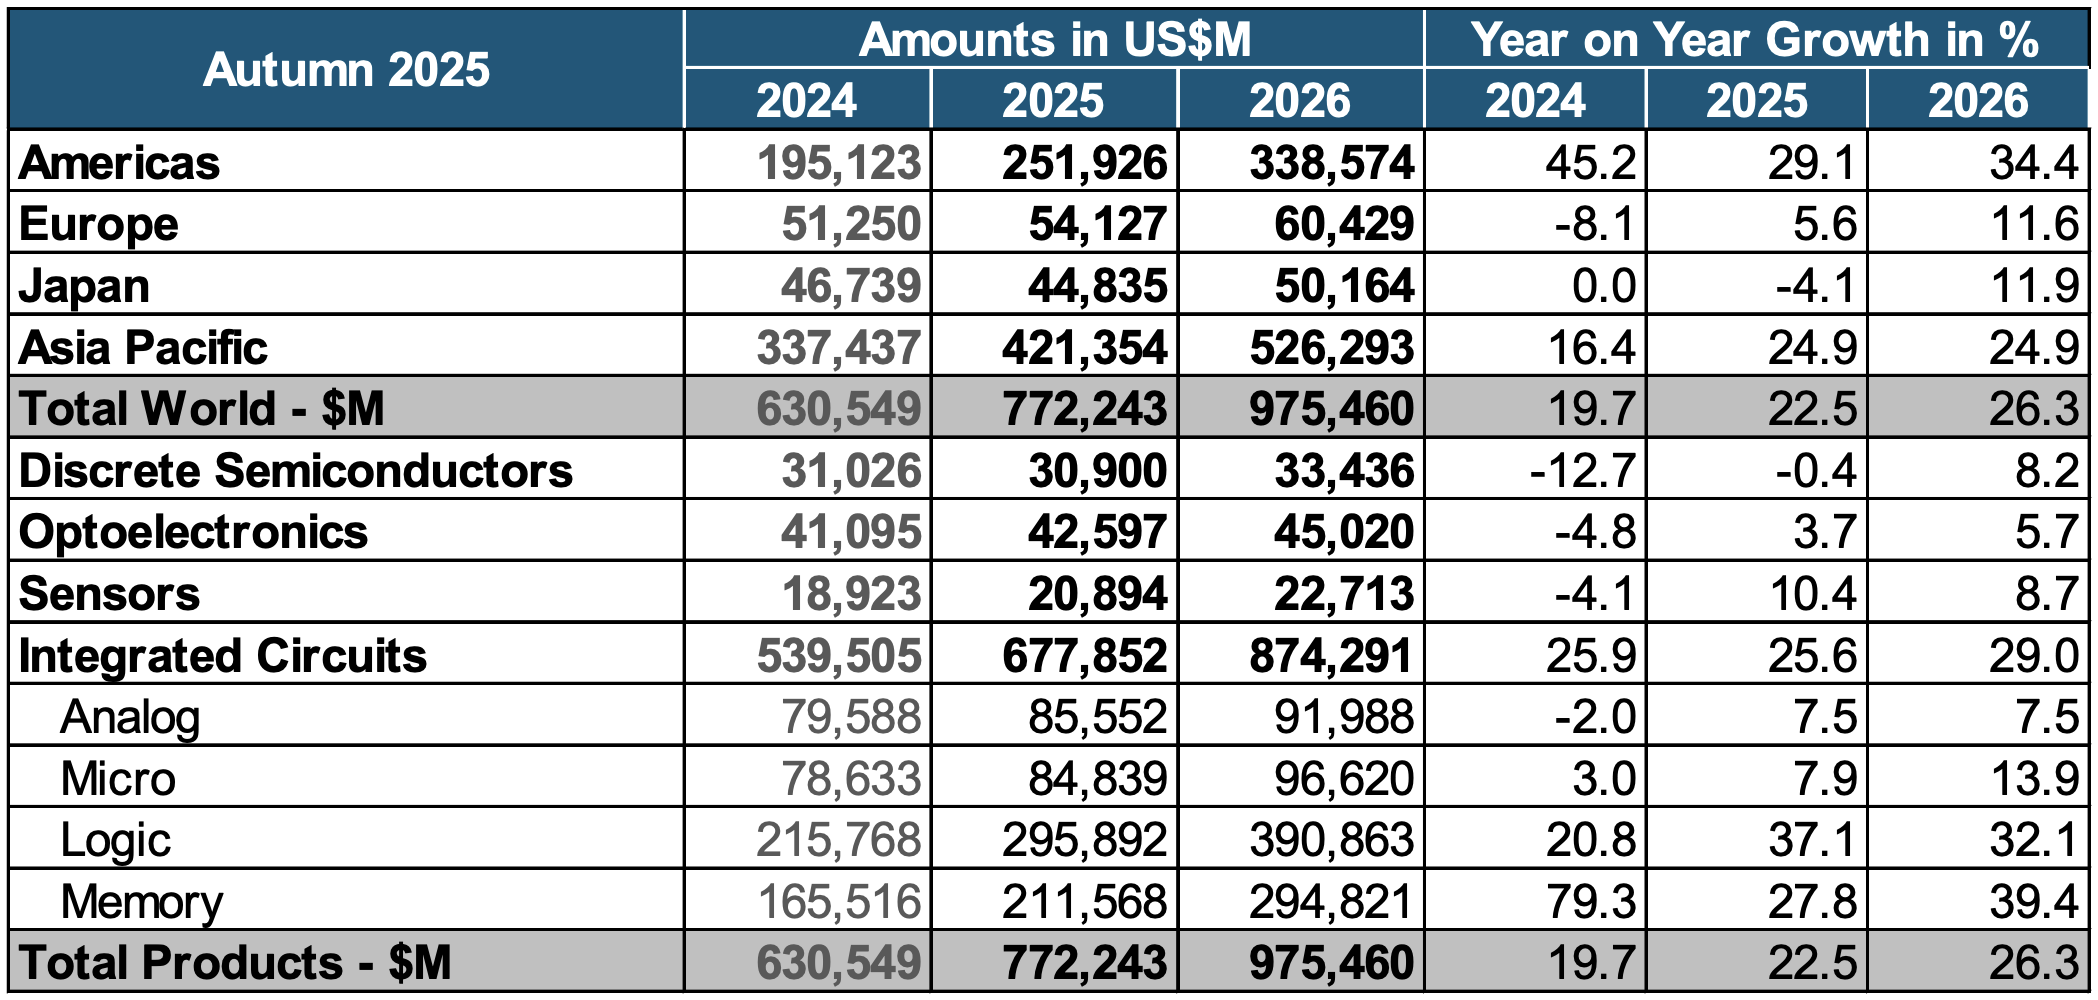
\includegraphics[width=.48\textwidth]{imgs/Table.png}
    \caption{WSTS Forecast Summary}
    \label{Table1}
\end{figure}

\section{The Companies}

In order to analyze which of the two is more important we can also check the big companies and see in which sector are they working and how big they are (in both terms of revenue and number of employees). A summary is shown in table \ref{tab:companies}, that groups some of the biggest electronic companies. 

\begin{table}[h]
    \centering
    \renewcommand{\arraystretch}{1.2}
    
    \rowcolors{2}{gray!10}{white}
    \begin{tabularx}{\columnwidth}{>{\raggedright\arraybackslash}X
                                    >{\centering\arraybackslash}p{2.0cm}
                                    >{\centering\arraybackslash}p{1.8cm}}
        \rowcolor{gray!60}
        \textcolor{white}{\textbf{Company}} &
        \textcolor{white}{\textbf{Revenue}} &
        \textcolor{white}{\textbf{Employees}} \\
        
        NVIDIA & 130.5 \$B & 36,000 \\
        Intel & 52.9 \$B & 85,100 \\
        AMD & 34.6 \$B & 31,000 \\
        Infineon & 14.7 €B & 57,000 \\
        Texas Instruments & 17.7 \$B & 33,000 \\
        Analog Devices & 11.0 \$B & 24,500 \\
        STMicroelectronics & 11.8 \$B & 49,157 \\
        
    \end{tabularx}
    \caption{Revenue and number of employees of selected semiconductor companies in 2025}
    \label{tab:companies}
\end{table}

\subsection{IC Companies}
In the table shown, almost all the companies are mostly IC-based. 

The first company in terms of revenue is NVIDIA, which sells IC devices as CPUs, GPUs and DPUs. \cite{nvidia2025annual} 

Intel is the one with the most number of employees, and it produces Microprocessors as well as SoCs, GPUs, NPUs, ASICSs and more. \cite{intel2025annual}

AMD is another fully IC company that in terms of business is similar to NVIDIA, selling CPUs, APUs and SoC. \cite{amd2025annual}

Texas Instruments normally sells Analog and Embedded Processing devices based on IC as well as Analog Devices that sells various IC devices in general for Mixed Signal purposes. \cite{ti2025annual} \cite{adi2025annual}

\subsection{Mixed Companies}
There are a lot of companies that sell both IC devices and Discrete devices. The first one that in the table is Infineon, from the financial report of 2025 we can estimate that approximatly 65\% of the revenues of the company comes from IC, while the discrete part takes around 30\%. \cite{infineon2025annual}

Also STMicroelectronics sells both the type of devices, having approximatly 10\% of discrete devices and 70\% of IC devices. \cite{stm2025annual}

\subsection{Discrete Circuits Companies}
Almost all the comanies work at least a part with IC devices, some exeptions are Nexperia and Vishay for example, both focused on devices as MOSFETs, Diodes, BJTs and more.

\section{Conclusion}
In conlusion, considering the data both from the market and from the single companies we can say that the majority of the elcectronic market is based on IC devices.

On the company side, we can surely say that given the big amount of emplyees and the large amount of IC devices, the request of IC expert is surely higher than the discrete one.
%%%%%%%%%%%%%%%%%%%%%%%%%%%%%%%%%%%%%%%%%
%             BIBLIOGRAPHY
%%%%%%%%%%%%%%%%%%%%%%%%%%%%%%%%%%%%%%%%%
\bibliographystyle{plain}
\bibliography{references}

\end{document}
